\documentclass[11pt]{article}
\usepackage{amsmath,amssymb,amsthm}
\usepackage{graphicx}
\usepackage{mathtools}

\addtolength{\evensidemargin}{-.5in}
\addtolength{\oddsidemargin}{-.5in}
\addtolength{\textwidth}{0.8in}
\addtolength{\textheight}{0.8in}

\title{ CS 224n: Assignment \#1 }
\author{Kristian Hartikainen}
\date{\today}
\pagestyle{myheadings}

\newcommand{\R}{\mathbb{R}}

\begin{document}
\maketitle

\section{Softmax}
\subsection*{(a)}
Softmax is invariant to constant offsets in the input:

\begin{equation*}
  \label{eq:softmax-constant-invariant}
  \begin{split}
    softmax(x)_{i} &= \frac{ e^{ x_{i} }       }{ \sum_{j}{ e^{ x_{j} }} }
                    = \frac{ e^{ x_{i} }       }{ \sum_{j}{ e^{ x_{j} }}} \frac{e^{c}}{{e^{c}}} \\
                 &= \frac{ e^{ x_{i} } e^{c} }{ \sum_{j}{ e^{ x_{j} } e^{c}}}
                  = \frac{ e^{ x_{i} + c }   }{ \sum_{j}{ e^{ x_{j} + c } } } \\
                 &= softmax(x + c)_{i}
  \qedhere
  \end{split}
\end{equation*}

\section{Neural Network Basics}
\subsection*{(a)}
\begin{equation*}
  \label{eq:sigmoid-gradient}
  \begin{split}
    \frac{ \partial }{ \partial x } \sigma(x)
      &= \frac{ \partial }{ \partial x } \frac{ 1 }{ 1 + e^{-x} } \\
      &= -1*(1 + e^{-x})^{-2} * \frac{ \partial }{ \partial x } (1+e^{-x}) \\
      &= -\frac{ -e^{-x} }{ (1 + e^{-x})^{2} } \\
      &=  \frac{ e^{-x} + 1 - 1 }{ (1 + e^{-x})^{2} } \\
      &=  \frac{ 1 + e^{-x} - 1 }{ 1 + e^{-x} } \frac{ 1 }{ 1 + e^{-x} } \\
      &=  (1 - \frac{ 1 }{ 1 + e^{-x} }) \frac{ 1 }{ 1 + e^{-x} } \\
      &=  (1 - \sigma(x)) \sigma(x) \\
  \qedhere
  \end{split}
\end{equation*}

\subsection*{(b)}
Let $\hat{y} = softmax(\theta)$ and $CE(y, \hat{y}) = -\sum_{i}{y log(\hat{y})}$. Then,

\begin{align*}
    \frac{ \partial }{ \partial \theta_{k} } CE(y, \hat{y})
      &= \frac{ \partial }{ \partial \theta_{k} } -\sum_{i}{y_i log(\hat{y}_i)} \\
      &= -\sum_{i}{y_i \frac{ \partial }{ \partial \theta_{k} } log(\hat{y}_i)} \\
      &= -\sum_{i}{y_i \frac{ \partial }{ \partial \theta_{k} } log(\frac{e^{\theta_i}}{\sum_{j}{e^{\theta_j}}})} \\
      &= -\sum_{i}{y_i \frac{ \partial }{ \partial \theta_{k} } (log(e^{\theta_i}) - log(\sum_{j}{e^{\theta_j}}))} \\
      &= -\sum_{i}{y_i \frac{ \partial }{ \partial \theta_{k} } (\theta_i - log(\sum_{j}{e^{\theta_j}}))} \\
      &= -\sum_{i}{y_i (\frac{ \partial \theta_{i} }{ \partial \theta_{k} } - \frac{ \partial }{ \partial \theta_{k} }log(\sum_{j}{e^{\theta_j}}) )} \\
      &= -\sum_{i}{y_i (\mathbf{1}_{i=k} - \frac{1}{\sum_{j}{e^{\theta_j}}} \sum_{j}{\frac{ \partial }{ \partial \theta_{k} } e^{\theta_j}} )} \\
      &= -\sum_{i}{y_i (\mathbf{1}_{i=k} - \frac{ e^{\theta_k} }{\sum_{j}{e^{\theta_j}}} )} \\
      &= -\sum_{i}{y_i (\mathbf{1}_{i=k} - \hat{y}_k )} \\
      &= -y_k(1 - \hat{y}_k) + \sum_{i \neq k}{y_{i}\hat{y}_{k}} \\
      &= -y_k + y_k\hat{y}_k + \sum_{i \neq k}{y_{i}\hat{y}_{k}} \\
      &= -y_k + \sum_{i}{y_{i}\hat{y}_{k}} && \sum_{i}y_{i} = 1\\
      &= \hat{y}_{k} - y_k
\end{align*}

Thus,
\begin{align*}
      \frac{ \partial }{ \partial \theta } CE(y, \hat{y}) = \hat{y} - y
\end{align*}


\subsection*{(c)}
Figure~\ref{fig:nn-computation-graph} represents a computational graph for a one-hidden-layer neural network with sigmoid non-linearity in the hidden units and cross-entropy loss for softmax output units. Given network inputs $X \in \R^{1 \times D_{in}}$ and labels $y \in \R^{1 \times D_{out}}$, we define the output $\hat{y}$ as follows:

\begin{figure}
  \centering
  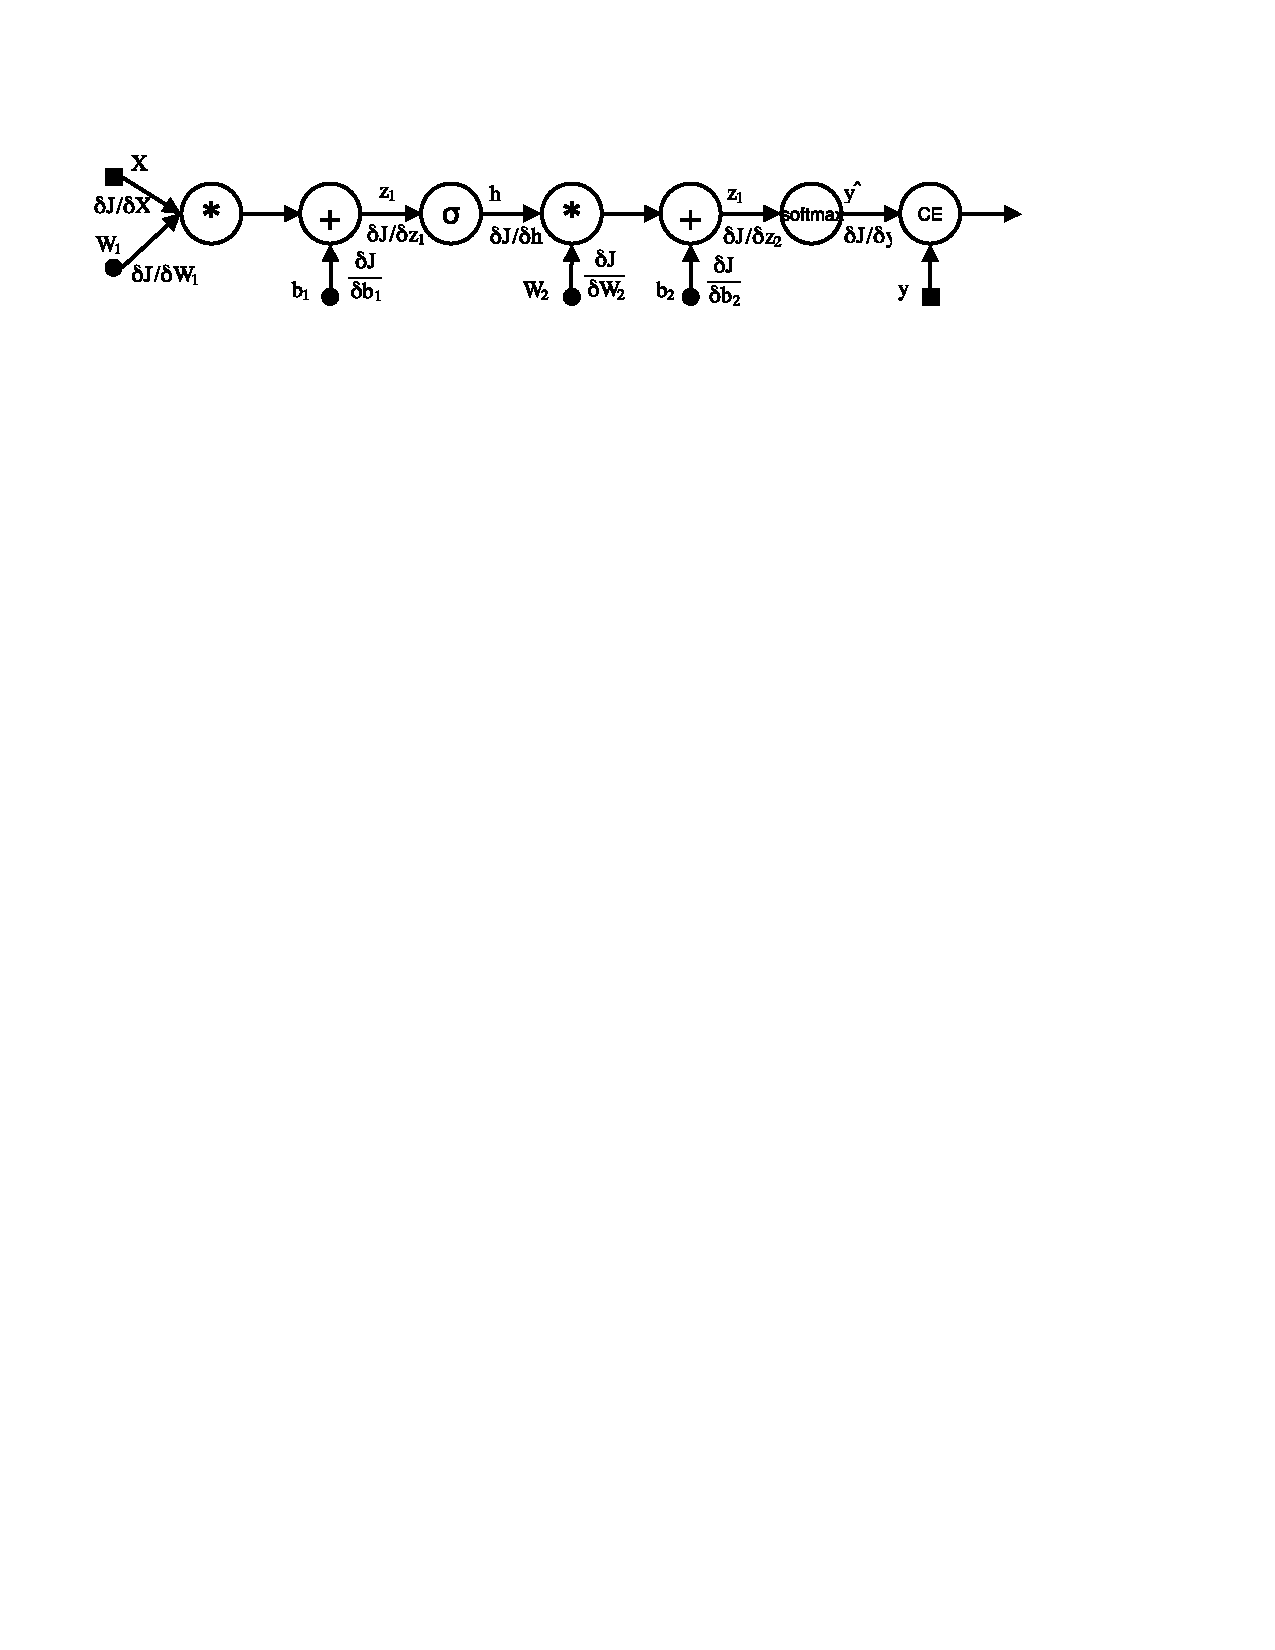
\includegraphics[width=\textwidth]{1-layer-network-forward-backward.pdf}

  \caption{The computational graph for 1-layer neural network with sigmoid non-linearity. The forward pass computation flows from left to right with solid arrow heads. Black symbols represent the inputs, parameters, and temporary variables of the network. The backward pass computation flows from right to left, with the red symbols representing the gradients flowing back from the loss function J to the inputs and parameters.}
  \label{fig:nn-computation-graph}
\end{figure}

\begin{equation*}
  \label{eq:forward-pass}
  \begin{split}
    \hat{y} &= softmax(z_{2}) \\
    z_{2} &= hW_{2} + b_{2} \\
    h &= \sigma(z_{1}) \\
    z_{1} &= XW_{1} + b_{1}
  \end{split}
\end{equation*}

Given the output $\hat{y}$, the cross-entropy loss for the network is defined as:

\begin{equation*}
  \label{eq:CE-loss}
  \begin{split}
    J(\theta) = CE(y, \hat{y}) = - \sum_{i} y_{i} log(\hat{y}_{i})
  \end{split}
\end{equation*}

The gradients of the network can be defined using chain-rule. Starting from $\frac{\partial J}{\partial z_{2}} = \frac{\partial CE(y, \hat{y})}{\partial z_{2}} = y - \hat{y}$ we get derivatives for $J$ w.r.t. $h$ and $z_{2}$ as follows:

\begin{equation*}
  \label{eq:temp-grads}
  \begin{split}
    \frac{\partial J}{\partial h} &= \frac{\partial J}{\partial z_{2}}\frac{\partial z_{2}}{\partial h} = (y - \hat{y}) W_{2}^{T}
    \\
    \frac{\partial J}{\partial z_{1}} &= \frac{\partial J}{\partial h}\frac{\partial h}{\partial z_{1}} = (y - \hat{y}) W_{2}^{T} diag(\sigma'(z_{1}))
  \end{split}
\end{equation*}

And the derivative w.r.t. the network parameters $W_{1}$, $b{1}$, $W_{2}$ and $b_{2}$ and input $X$ as follows:

\begin{equation*}
  \label{eq:param-grads}
  \begin{split}
    \frac{\partial J}{\partial b_{2}} &= \frac{\partial J}{\partial z_{2}}\frac{\partial z_{2}}{\partial b_{2}} = (y - \hat{y}) [1 1 \hdots 1]^{T} = \sum_{i}{y_{i} - \hat{y}_{i}}
    \\
    \frac{\partial J}{\partial W_{2}} &= \frac{\partial J}{\partial z_{2}}\frac{\partial z_{2}}{\partial W_{2}} = (y - \hat{y}) h_{1}.
    \\
    \frac{\partial J}{\partial b_{1}} &= \frac{\partial J}{\partial z_{1}}\frac{\partial z_{1}}{\partial b_{1}} = \sum_{i}{(\frac{\partial J}{\partial z_{1}})_{i}}
    \\
    \frac{\partial J}{\partial W_{1}} &= \frac{\partial J}{\partial z_{1}}\frac{\partial z_{1}}{\partial W_{1}} = (y - \hat{y}) W_{2}^{T} diag(\sigma'(z_{1})) X
    \\
    \frac{\partial J}{\partial X} &= \frac{\partial J}{\partial z_{1}}\frac{\partial z_{1}}{\partial X} = (y - \hat{y}) W_{2}^{T} diag(\sigma'(z_{1})) W_{1}^{T}
  \end{split}
\end{equation*}

\subsection*{(d)}
Assuming the input for this neural network is $D_{x}$-dimensional, the output is $D_{y}$-dimensional, and there are H hidden units, the contains $D_{x}H + H + HD_{y} + D_{y}$ parameters.

\section{word2vec}
\subsection*{(a)}
\subsection*{(b)}
\subsection*{(c)}
\subsection*{(d)}

\section{Sentiment Analysis}
\subsection*{(b)}

\subsection*{(d)}

\end{document}
%%% Local Variables:
%%% mode: latex
%%% TeX-master: t
%%% End:
